\subsection{Respuesta al escalón de la fuente de tensión $V_d$}

    Con las condiciones nominales se obtuvo la respuesta al escalón observable en la Figura 
    \ref{fig:respuesta_escalon}. Se observa un sobrepico de 
    aproximadamente 1,8 V, lo que nos hace pensar que hay un sistema subamortiguado en algún lado. Para caracterizarlo en más profundidad, se obtuvo el tiempo de establecimiento del 5\% de 
    la respuesta estacionaria, aproximadamente 1,3 ms (desde que comienza la pendiente por comienzo de carga de los capacitores hasta que la salida se mantiene estable 
    dentro de la banda de tensiones entre 4,5 V y 4 V aproximadamente).
    \begin{figure}[H]
        \centering
        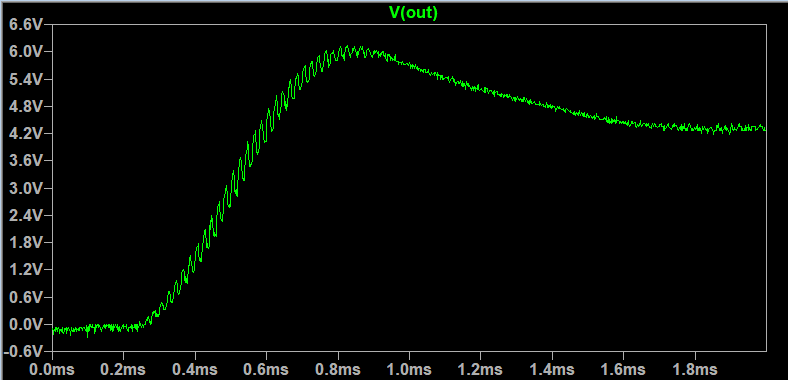
\includegraphics[width=0.7\textwidth]{imagenes/tp3_c.png}
        \caption{Respuesta al escalón de la fuente de tensión $V_d$. Se observa un sobrepico ya mencionado. La tensión medida es sobre la resistencia de carga $R_L$. }
        \label{fig:respuesta_escalon}
     \end{figure}